\subsection{Establecimiento}

A continuación, se expone un análisis de los costos e inversiones requeridos para la puesta en marcha de la empresa, abarcando aspectos como el diseño, desarrollo e implementación del software. Este análisis contempla los recursos económicos, humanos, administrativos y pre-operativos necesarios para iniciar las operaciones, detallados de la siguiente forma:

\subsubsection{Activos fijos tangibles}

Los activos fijos tangibles se clasifican en dos grandes áreas: la operacional y la administrativa, ambas esenciales para el arranque del proyecto. La tabla \ref{activosTangiles} muestra una descripción detallada de cada una:

    \vspace{2mm}
        \begin{minipage}{0.9\textwidth}
        \centering
        \captionof{table}[{Activos tangibles}]{Activos tangibles}
        \label{activosTangiles}
        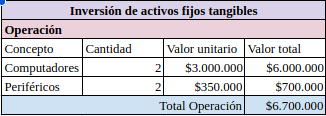
\includegraphics[width=0.9\textwidth]{Content/Images/AF/Establecimiento_tangibles.png}
        \footnote{Nota. \textup{Fuente : Autores.}}
        \end{minipage}

\subsubsection{Activos fijos intangibles}

Los activos fijos intangibles corresponden a los trámites financieros y legales que la empresa debe gestionar, como se describe en la tabla \ref{Establecimiento_intangibles}.

\vspace{2mm}
        \begin{minipage}{0.9\textwidth}
        \centering
        \captionof{table}[{Activos intangibles}]{Activos intangibles}
        \label{Establecimiento_intangibles}
        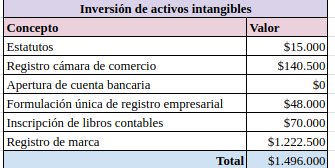
\includegraphics[width=0.9\textwidth]{Content/Images/AF/Establecimiento_intangibles.png}
        \footnote{Nota. \textup{Fuente : Autores.}}
        \end{minipage}

\subsubsection{Total activos fijos}
La tabla \ref{Establecimiento_totalActivos} resume la inversión total necesaria para adquirir los activos fijos y el capital de trabajo indispensable para ejecutar el proyecto.

\vspace{2mm}
        \begin{minipage}{0.9\textwidth}
        \centering
        \captionof{table}[{Total de activos}]{Total de activos}
        \label{Establecimiento_totalActivos}
        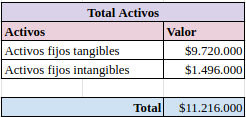
\includegraphics[width=0.9\textwidth]{Content/Images/AF/Establecimiento_totalActivos.png}
        \footnote{Nota. \textup{Fuente : Autores.}}
        \end{minipage}

\subsubsection{Financiamiento}
En la tabla \ref{Establecimiento_Financiacion} se detalla la inversión necesaria para la etapa inicial del proyecto, la cual debe analizarse considerando tanto el aporte de capital social como el financiamiento externo.

\vspace{2mm}
        \begin{minipage}{0.9\textwidth}
        \centering
        \captionof{table}[{Financiacion}]{Financiacion}
        \label{Establecimiento_Financiacion}
        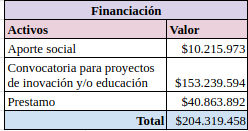
\includegraphics[width=0.9\textwidth]{Content/Images/AF/Establecimiento_Financiacion.png}
        \footnote{Nota. \textup{Fuente : Autores.}}
        \end{minipage}
